\documentclass[11pt, a4paper]{article}

\usepackage{amsmath}
\usepackage{amsfonts} %Matheschriften
\usepackage{amssymb} %Mathesymbole
%\usepackage{mathptmx} % Einstellung für Schriften und Sonderzeichen in mathematischen Umgebungen
                        % ändert SChriftfont
\usepackage{wasysym} % Stellt diverse Sonderzeichen bereit
\usepackage{siunitx}
\usepackage{float}
\usepackage{microtype}
\usepackage{graphicx}
\usepackage{hyperref}
\usepackage{xcolor}
\usepackage[section]{placeins}
% allows for temporary adjustment of side margins
\usepackage{changepage}
\usepackage{rotating}


\usepackage[ngerman]{babel}
\addto\captionsngerman{%
 \renewcommand{\abstractname}{Einleitung}}

\title{Versuch 4: Transistor}
\author{Team 2-13: Jascha Fricker, Benedict Brouwer}

\begin{document}
    \maketitle

    \tableofcontents

    \newpage
\section{Introduction}
In this experiment we examined the properties of a bipolar transistor in combination with an emitter circuit. Therby we measured the characteristic curve 
of the transistor and tested different konfigurations of the emittercircuit.
\section{Theorie}

\section{execution}
\begin{figure}[h]
    \centering
    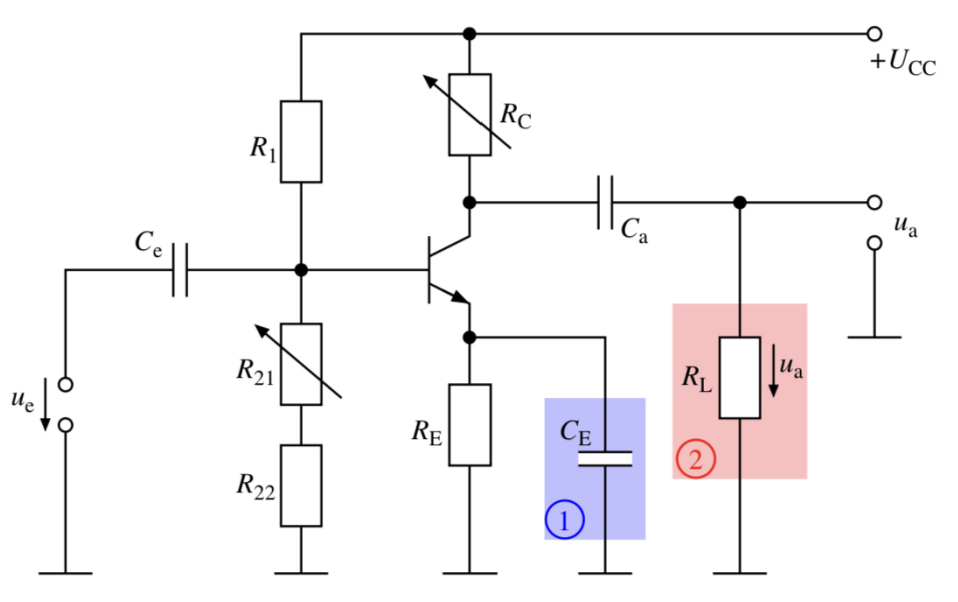
\includegraphics[width=0.8\textwidth]{bilder/Emitter circuit.png}
    \caption{emittercircuit:\\
    $R_1$ = 47 \si{\kilo\ohm}, $R_{22}$ = 100 \si{\ohm},$R_E$ = 10 \si{\kilo\ohm}, $C_e$ = 47 \si{\micro\farad},$C_a$ = 470 \si{\micro\farad}, $U_{CC}$ = 9 \si{\volt} 
    $R_{12}$: potentiometer for the workingpoint, $R_C$: potentiometer 0 - 10 \si{\kilo\ohm}, $u_e$: inputvoltage, $u_a$: outputvoltage
    
    }
    \label{im:Emcir}
\end{figure}

\subsection{workingpoint}
A bipolar transistor has a specific basevoltage range (the so called workingpoint) in wich it behaves approxmately linear. This workingpoint
is tuned by setting the resistance at the potentiometer $R_{12}$ \ref{im:Emcir}[see circuit diagram] to a point whereby the outputamplitude $u_a$ is maximal and the signal is not distorted.
To tune the workingpoint, the loadresistor $R_L$ was removed and a sinusoidal frequency of 5.5 \si{\kilp\hertz} was applied. 
$U_{\text{BE}}$, $U_{\text{CE}}$, $I_{\text{C}}$ where measured with varying $R_{\text{C}}$ for further evaluation.
\subsection{Amplification of the emittercircuit}
To further examine the emittercircuit \ref{im:Emcir}[see circuit diagram] the amplidude quotionet $u_a / u_e$ was measured for varying $R_{\text{C}}$ in different circuit configurations:\\
1. with capacitor $C{\text{E}}$ but without resistor $R_{\text{L}}$
2. without capacitor $C{\text{E}}$ and without resistor $R_{\text{L}}$
3. with capacitor $C{\text{E}}$ and resistor $R_{\text{L}}$
\subsection{Frequency response}
In this experiment the input frequency was varied from 6 \si{\hertz} - 250 \si{\kilo\hertz} to measure the phaseshift and the amplidude quotionet $u_a / u_e$. 
Therby circuit \ref{im:Emcir} with an collectorresistor of $R_{\text{C}}$ was used.
\subsection{characteristic curve}
\begin{figure}[h]
    \centering
    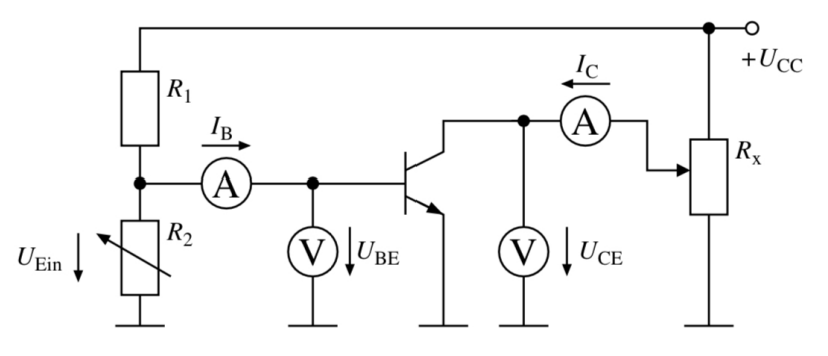
\includegraphics[width=0.8\textwidth]{bilder/characteristicCurve.png}
    \caption{characteristic curve}
    \label{im:Charcurcir}
\end{figure}

\section{results}

\begin{table}[!ht]
    \centering
    \begin{tabular}{l|l|l|l}
    
        $R_{\text{C}}$ in \si{\kilo\ohm}  & $U_{\text{BE}}$ in \si{\volt} & $U_{\text{CE}}$ in \si{\volt} & $I_{\text{C}}$ in \si{\milli\ampere}  \\ \hline
        1 & 0,57 & 7,86 & 0,58 \\ \hline
        5 & 0,57 & 5,53 & 0,58 \\ \hline
        10 & 0,57 & 3,22 & 0,58 \\ 
    \end{tabular}
\end{table}


\bibliographystyle{plain}
\bibliography{literature}

\end{document}

